%%%%%%%%%%%%%%%%%%%%%%%%%%%%%%%%%%%
\chapter{Métricas de Evolução das Comunidades Científicas}\label{apendice:metricas_evolucao_comunidades}
%%%%%%%%%%%%%%%%%%%%%%%%%%%%%%%%%%%

Neste apêndice apresentamos as métricas das demais conferências, separada entre três grupos. O grupo A é constituído pelas conferências
CIKM, CHI, KDD, SAC e SIGCOMM, o grupo B pelas conferências CSS, MICRO, MM, MOBICOM e SIGDOC, e o grupo C pelas conferências
HSCC, ICSE, ISCA, SIGCSE, SIGGRAPH e SIGMETRICS.

\begin{figure}[!htb]
  \begin{center}
  \subfloat[Assortatividade final - Grupo A]{%
    \label{fig:assortativity_1_in_1_apendice_grupa_a}
    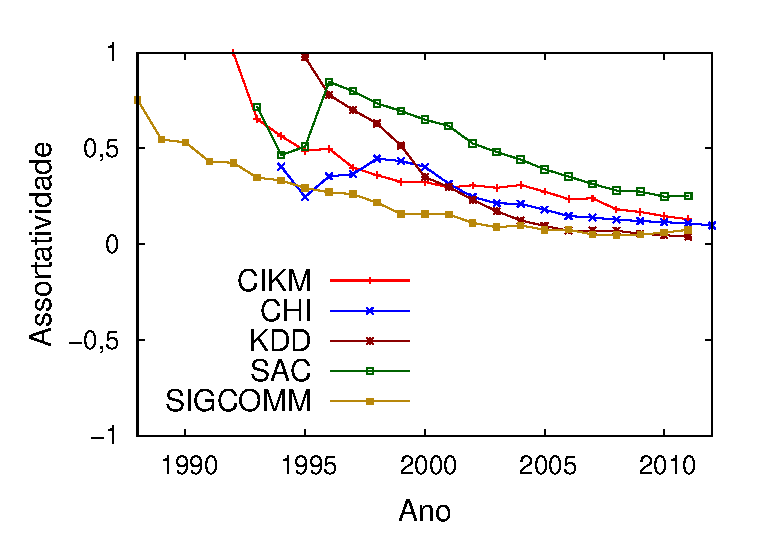
\includegraphics[scale=.6]{../graficos/sigs_metricas_acumuladas_1_em_1_ano/pt_BR/assortatividade_grupo_temporal_web_apendice_1.eps}
  }%
  \subfloat[Assortatividade por janela - Grupo A]{%
    \label{fig:assortativity_slide_window_apendice_grupa_a}
    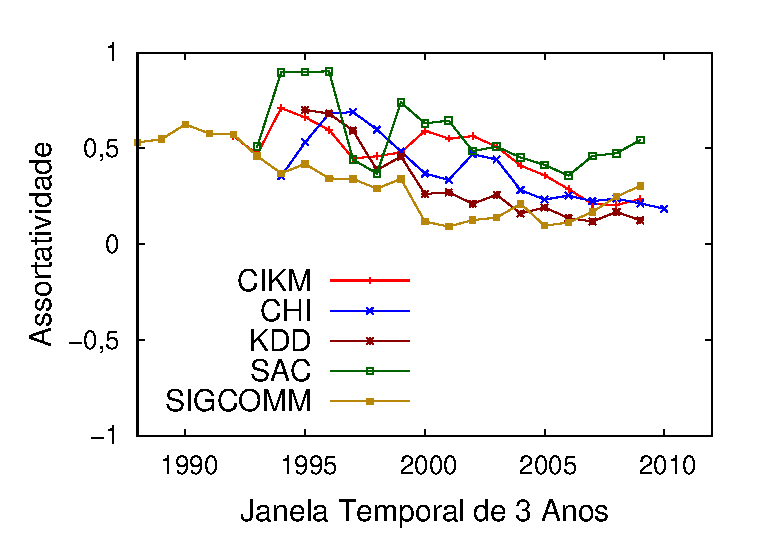
\includegraphics[scale=.6]{../graficos/core_over_time/metricas_tradicionais/pt_BR/assortatividade_slide_window_grupo_temporal_web_apendice_1.eps}
  }%
  \phantomcaption
  \end{center}
\end{figure}
\begin{figure}[!htb]
  \begin{center}
  \ContinuedFloat
  \subfloat[Assortatividade final - Grupo B]{%
    \label{fig:assortativity_1_in_1_apendice_grupa_b}
    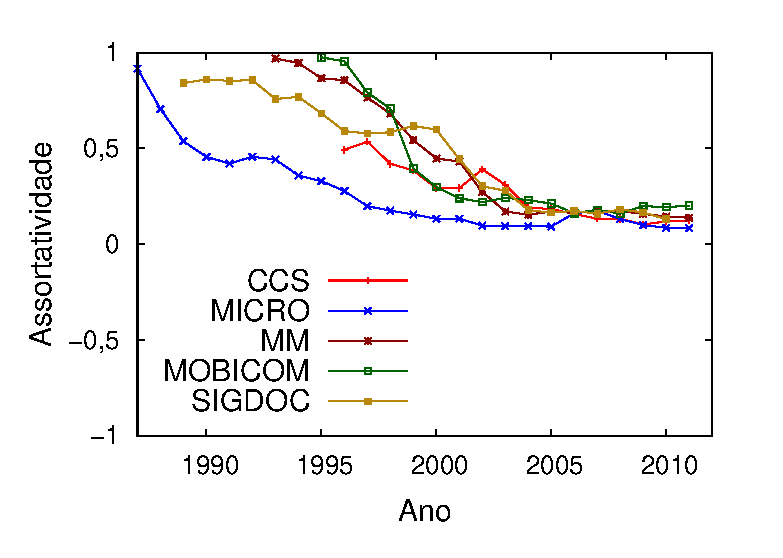
\includegraphics[scale=.6]{../graficos/sigs_metricas_acumuladas_1_em_1_ano/pt_BR/assortatividade_grupo_temporal_web_apendice_2.eps}
  }%
  \subfloat[Assortatividade por janela - Grupo B]{%
    \label{fig:assortativity_slide_window_apendice_grupa_b}
    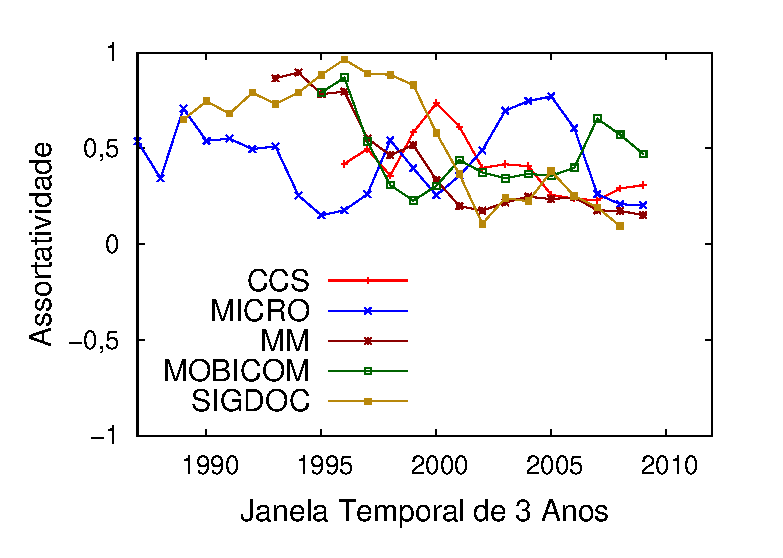
\includegraphics[scale=.6]{../graficos/core_over_time/metricas_tradicionais/pt_BR/assortatividade_slide_window_grupo_temporal_web_apendice_2.eps}
  }%
  \\
  \subfloat[Assortatividade final - Grupo C]{%
    \label{fig:assortativity_1_in_1_apendice_grupa_c}
    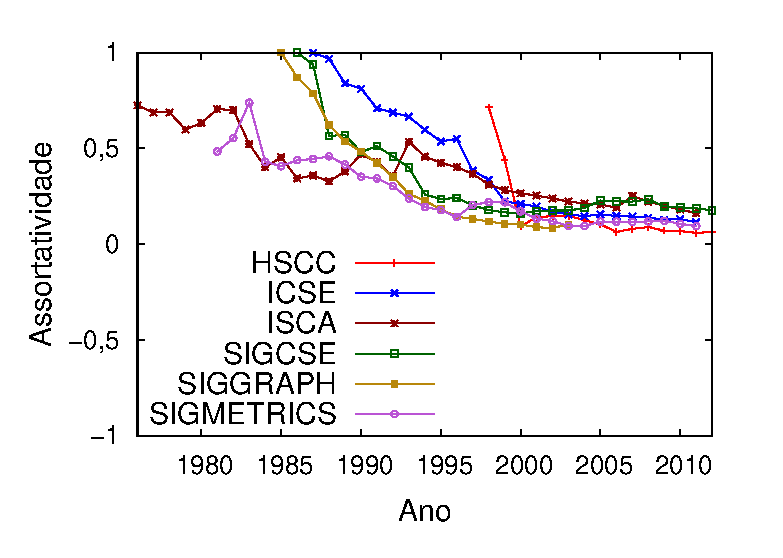
\includegraphics[scale=.6]{../graficos/sigs_metricas_acumuladas_1_em_1_ano/pt_BR/assortatividade_grupo_temporal_web_apendice_3.eps}
  }%
  \subfloat[Assortatividade por janela - Grupo C]{%
    \label{fig:assortativity_slide_window_apendice_grupa_c}
    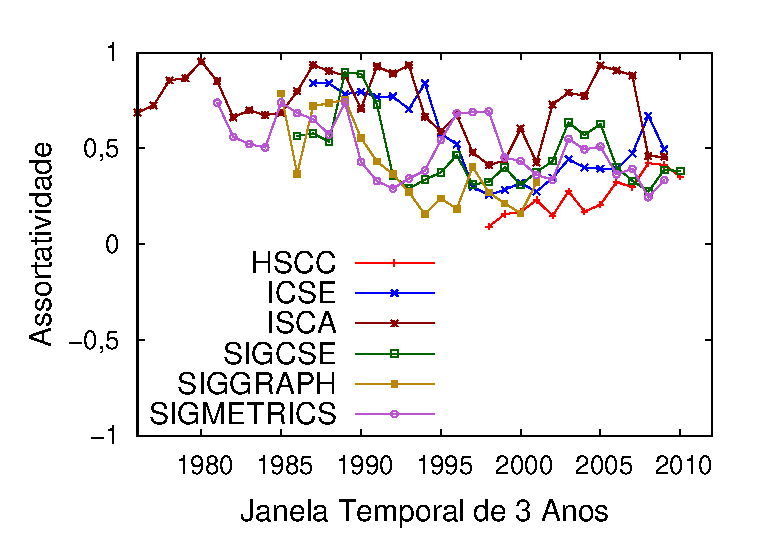
\includegraphics[scale=.6]{../graficos/core_over_time/metricas_tradicionais/pt_BR/assortatividade_slide_window_grupo_temporal_web_apendice_3.eps}
  }%
  \end{center}
  \caption{Assortatividade das comunidades científicas}
  \label{fig:metrics_assortativity_apendice}
\end{figure}


\begin{figure}[!htb]
  \begin{center}
  \subfloat[CMM final - Grupo A]{%
    \label{fig:average_shortest_1_in_1_apendice_grupa_a}
    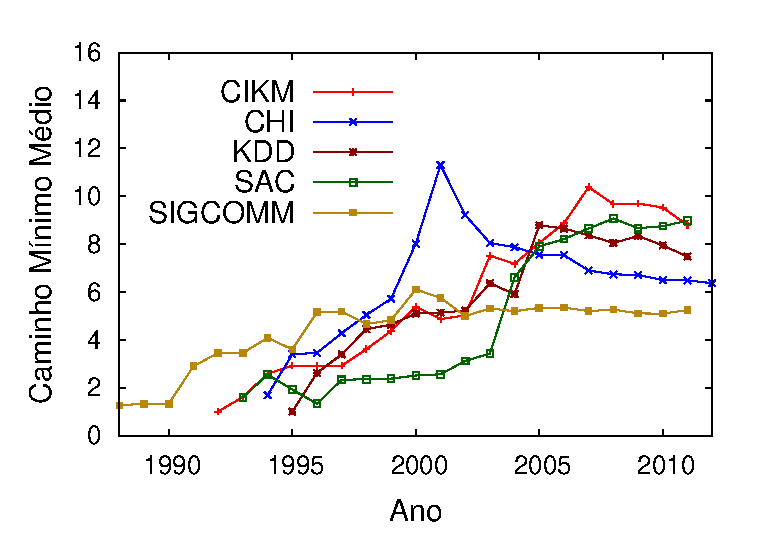
\includegraphics[scale=.6]{../graficos/sigs_metricas_acumuladas_1_em_1_ano/pt_BR/caminho_minimo_medio_grupo_temporal_web_apendice_1.eps}
  }%
  \subfloat[CMM por janela - Grupo A]{%
    \label{fig:average_shortest_slide_window_apendice_grupa_a}
    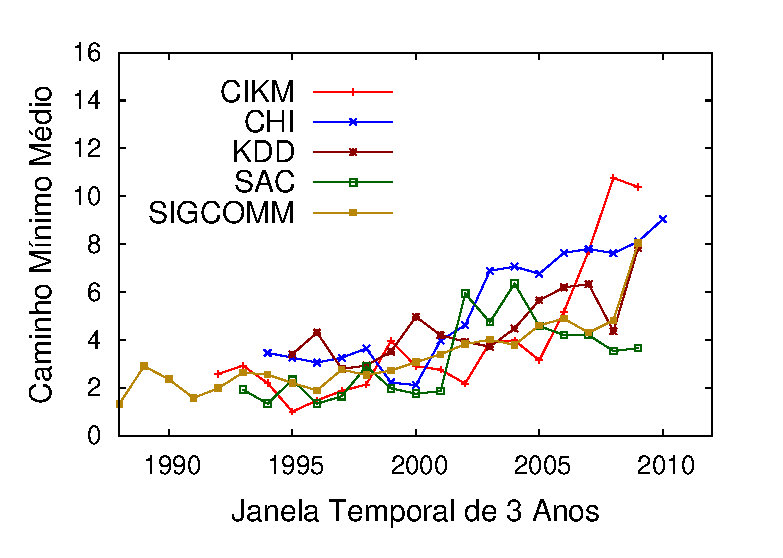
\includegraphics[scale=.6]{../graficos/core_over_time/metricas_tradicionais/pt_BR/caminho_minimo_medio_slide_window_grupo_temporal_web_apendice_1.eps}
  }%
  \phantomcaption
  \end{center}
\end{figure}
\begin{figure}[!htb]
  \begin{center}
  \ContinuedFloat
  \subfloat[CMM final - Grupo B]{%
    \label{fig:average_shortest_1_in_1_apendice_grupa_b}
    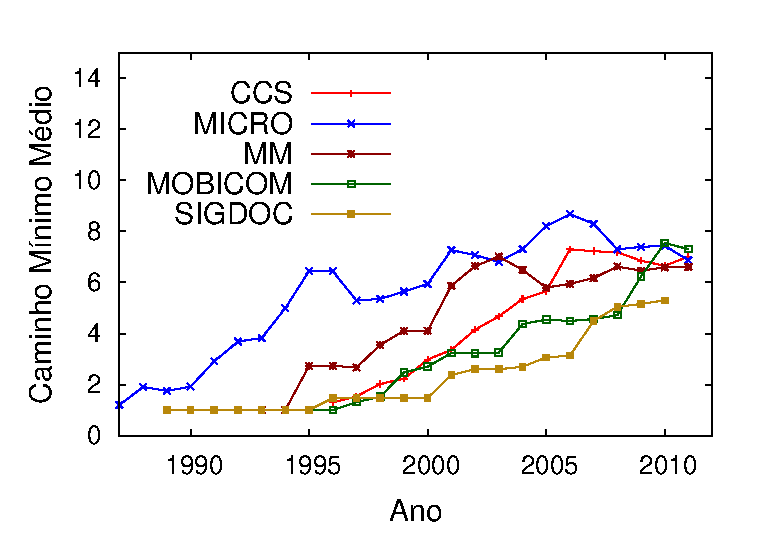
\includegraphics[scale=.6]{../graficos/sigs_metricas_acumuladas_1_em_1_ano/pt_BR/caminho_minimo_medio_grupo_temporal_web_apendice_2.eps}
  }%
  \subfloat[CMM por janela - Grupo B]{%
    \label{fig:average_shortest_slide_window_apendice_grupa_b}
    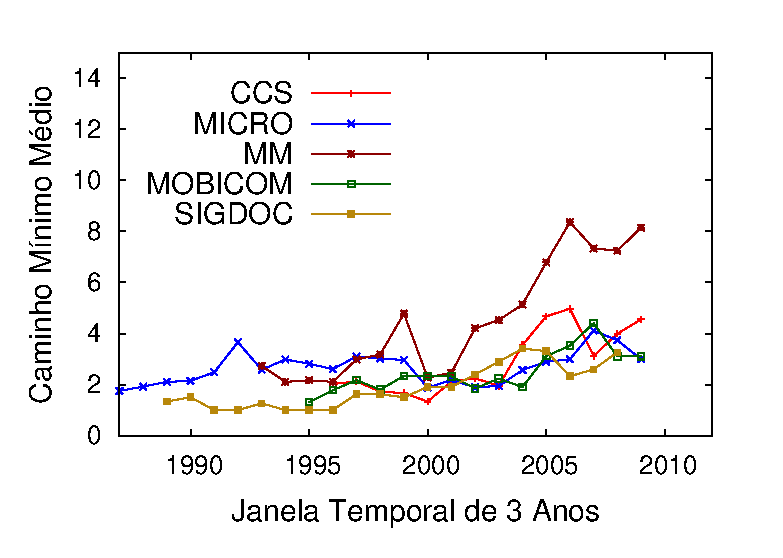
\includegraphics[scale=.6]{../graficos/core_over_time/metricas_tradicionais/pt_BR/caminho_minimo_medio_slide_window_grupo_temporal_web_apendice_2.eps}
  }%
  \\
  \subfloat[CMM final - Grupo C]{%
    \label{fig:average_shortest_1_in_1_apendice_grupa_c}
    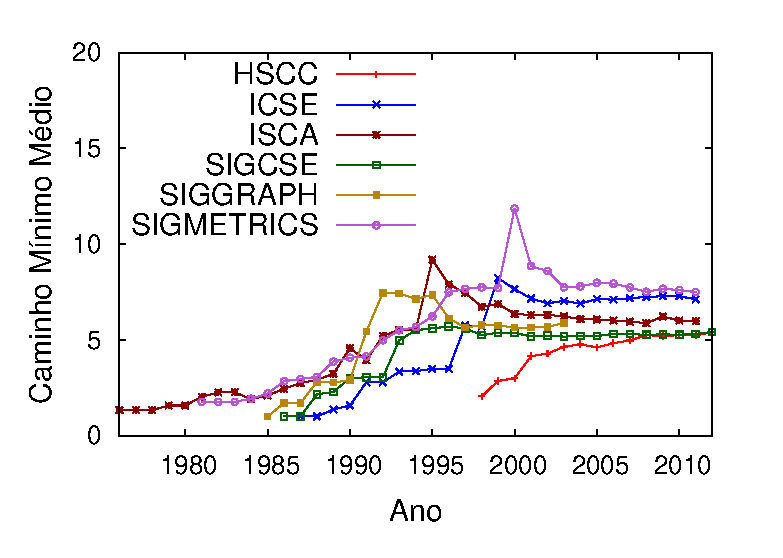
\includegraphics[scale=.6]{../graficos/sigs_metricas_acumuladas_1_em_1_ano/pt_BR/caminho_minimo_medio_grupo_temporal_web_apendice_3.eps}
  }%
  \subfloat[CMM por janela - Grupo C]{%
    \label{fig:average_shortest_slide_window_apendice_grupa_c}
    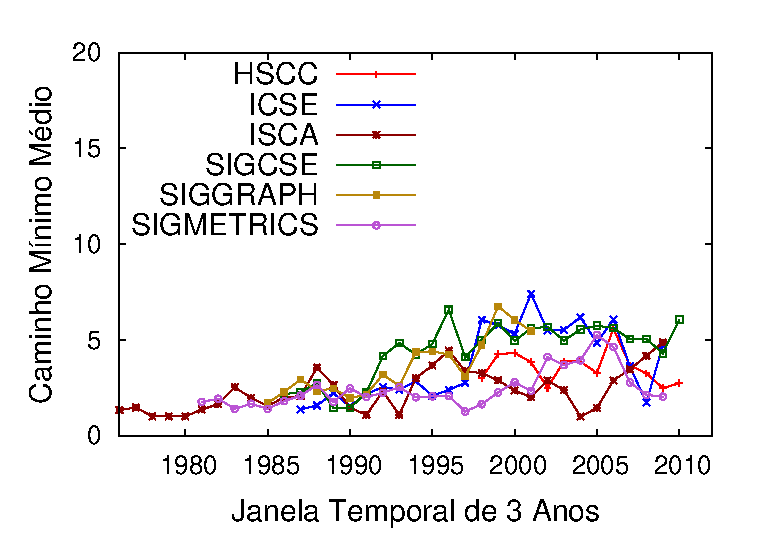
\includegraphics[scale=.6]{../graficos/core_over_time/metricas_tradicionais/pt_BR/caminho_minimo_medio_slide_window_grupo_temporal_web_apendice_3.eps}
  }%
  \end{center}
  \caption{Caminho mínimo médio das comunidades científicas}
  \label{fig:metrics_average_shortest_apendice}
\end{figure}


\begin{figure}[!htb]
  \begin{center}
  \subfloat[CA final - Grupo A]{%
    \label{fig:average_shortest_1_in_1_apendice_grupa_a}
    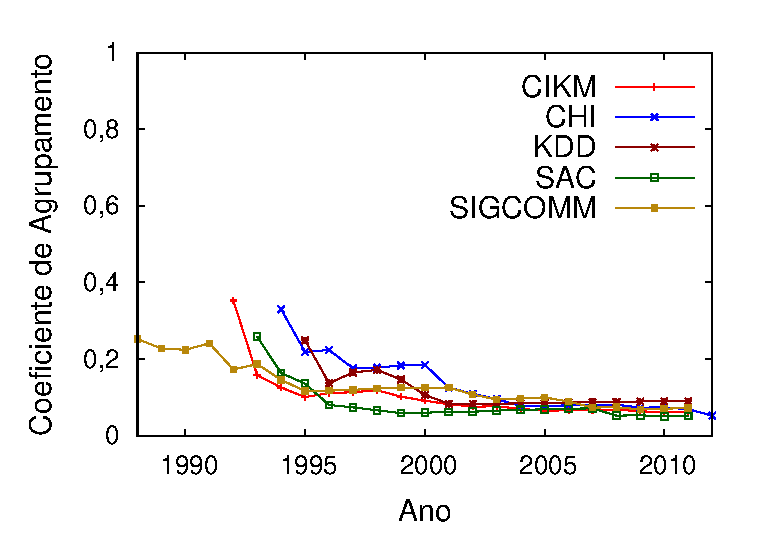
\includegraphics[scale=.6]{../graficos/sigs_metricas_acumuladas_1_em_1_ano/pt_BR/coeficiente_agrupamento_grupo_temporal_web_apendice_1.eps}
  }%
  \subfloat[CA por janela - Grupo A]{%
    \label{fig:average_shortest_slide_window_apendice_grupa_a}
    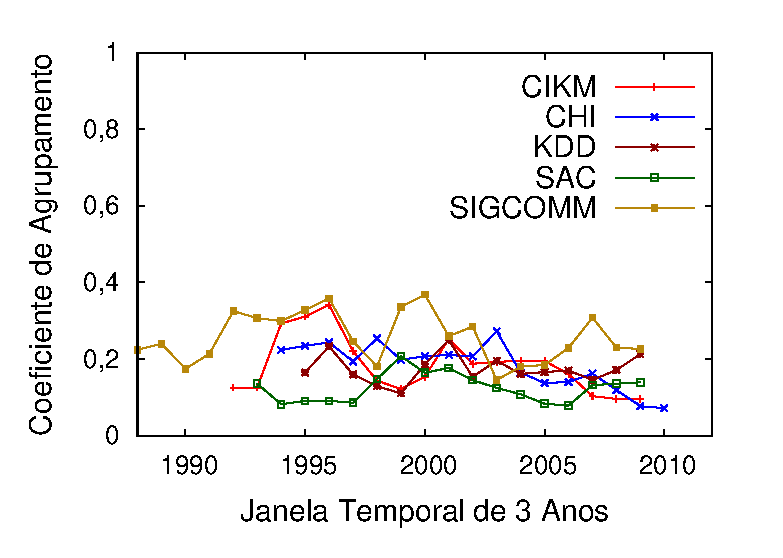
\includegraphics[scale=.6]{../graficos/core_over_time/metricas_tradicionais/pt_BR/coeficiente_agrupamento_slide_window_grupo_temporal_web_apendice_1.eps}
  }%
  \phantomcaption
  \end{center}
\end{figure}
\begin{figure}[!htb]
  \begin{center}
  \ContinuedFloat
  \subfloat[CA final - Grupo B]{%
    \label{fig:average_shortest_1_in_1_apendice_grupa_b}
    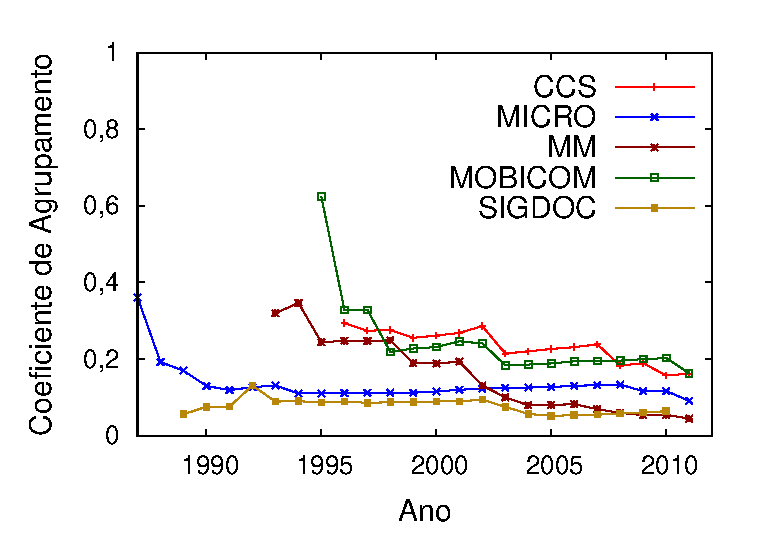
\includegraphics[scale=.6]{../graficos/sigs_metricas_acumuladas_1_em_1_ano/pt_BR/coeficiente_agrupamento_grupo_temporal_web_apendice_2.eps}
  }%
  \subfloat[CA por janela - Grupo B]{%
    \label{fig:average_shortest_slide_window_apendice_grupa_b}
    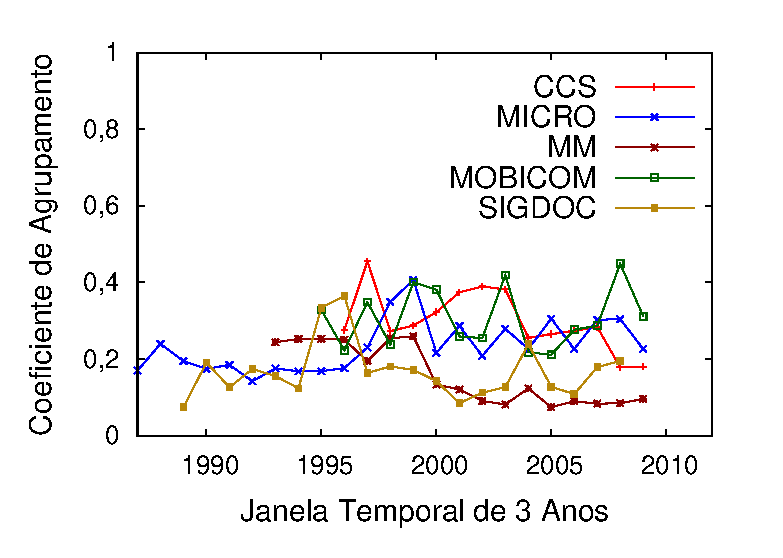
\includegraphics[scale=.6]{../graficos/core_over_time/metricas_tradicionais/pt_BR/coeficiente_agrupamento_slide_window_grupo_temporal_web_apendice_2.eps}
  }%
  \\
  \subfloat[CA final - Grupo C]{%
    \label{fig:average_shortest_1_in_1_apendice_grupa_c}
    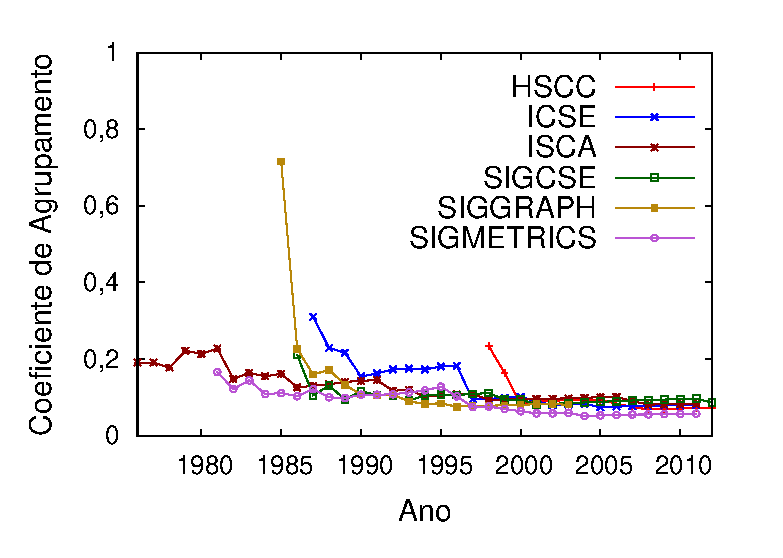
\includegraphics[scale=.6]{../graficos/sigs_metricas_acumuladas_1_em_1_ano/pt_BR/coeficiente_agrupamento_grupo_temporal_web_apendice_3.eps}
  }%
  \subfloat[CA por janela - Grupo C]{%
    \label{fig:average_shortest_slide_window_apendice_grupa_c}
    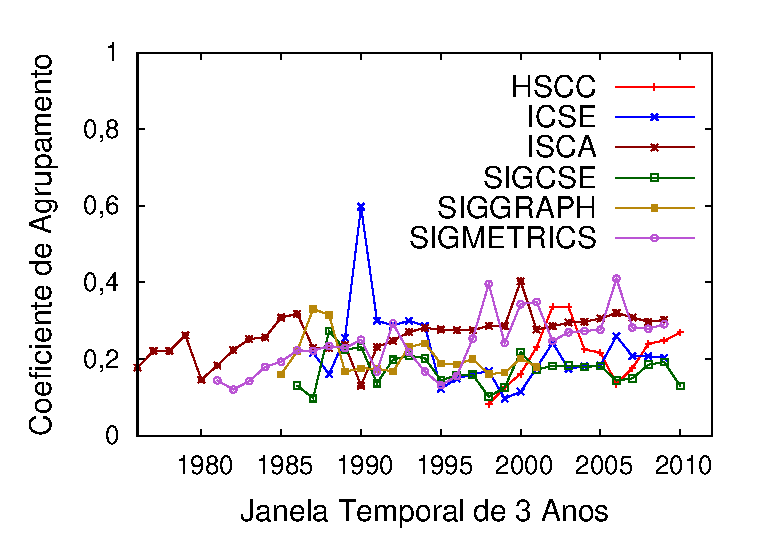
\includegraphics[scale=.6]{../graficos/core_over_time/metricas_tradicionais/pt_BR/coeficiente_agrupamento_slide_window_grupo_temporal_web_apendice_3.eps}
  }%
  \end{center}
  \caption{Coeficiente de agrupamento das comunidades científicas}
  \label{fig:metrics_average_shortest_apendice}
\end{figure}


\begin{figure}[!htb]
  \begin{center}
  \subfloat[Maior CFC final - Grupo A]{%
    \label{fig:average_shortest_1_in_1_apendice_grupa_a}
    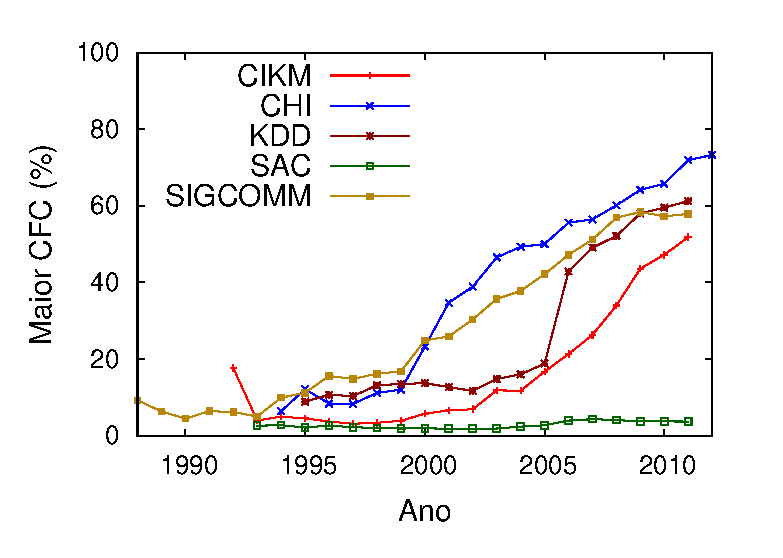
\includegraphics[scale=.6]{../graficos/sigs_metricas_acumuladas_1_em_1_ano/pt_BR/porcentagem_maior_componente_grupo_temporal_web_apendice_1.eps}
  }%
  \subfloat[Maior CFC por janela - Grupo A]{%
    \label{fig:average_shortest_slide_window_apendice_grupa_a}
    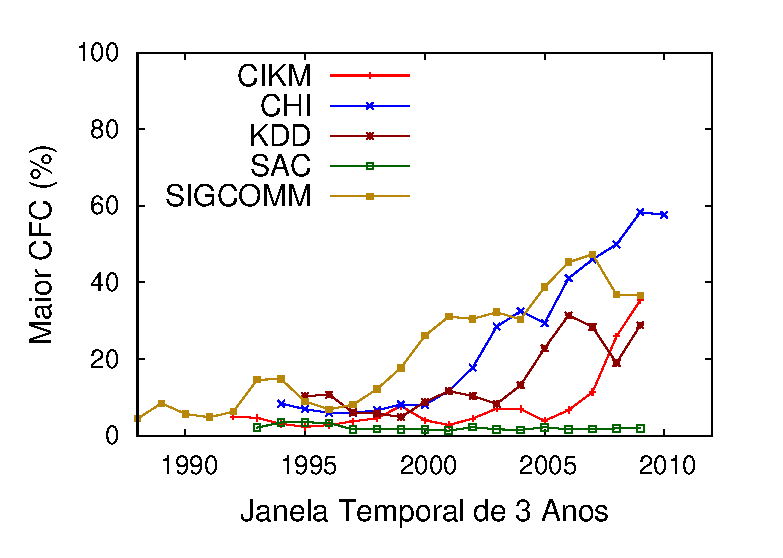
\includegraphics[scale=.6]{../graficos/core_over_time/metricas_tradicionais/pt_BR/porcentagem_maior_componente_slide_window_grupo_temporal_web_apendice_1.eps}
  }%
  \phantomcaption
  \end{center}
\end{figure}
\begin{figure}[!htb]
  \begin{center}
  \ContinuedFloat
  \subfloat[Maior CFC final - Grupo B]{%
    \label{fig:average_shortest_1_in_1_apendice_grupa_b}
    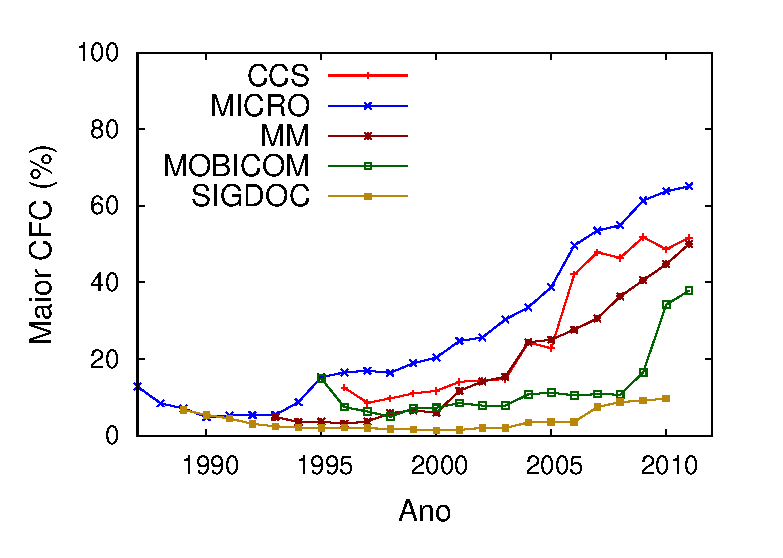
\includegraphics[scale=.6]{../graficos/sigs_metricas_acumuladas_1_em_1_ano/pt_BR/porcentagem_maior_componente_grupo_temporal_web_apendice_2.eps}
  }%
  \subfloat[Maior CFC por janela - Grupo B]{%
    \label{fig:average_shortest_slide_window_apendice_grupa_b}
    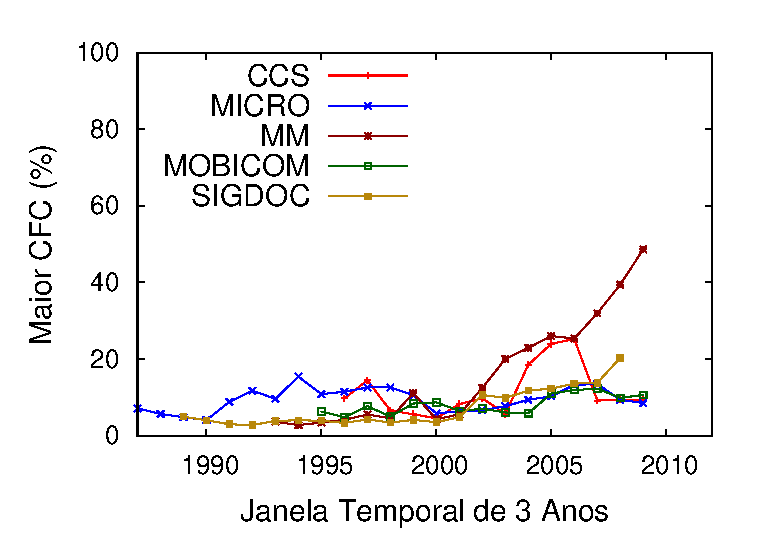
\includegraphics[scale=.6]{../graficos/core_over_time/metricas_tradicionais/pt_BR/porcentagem_maior_componente_slide_window_grupo_temporal_web_apendice_2.eps}
  }%
  \\
  \subfloat[Maior CFC final - Grupo C]{%
    \label{fig:average_shortest_1_in_1_apendice_grupa_c}
    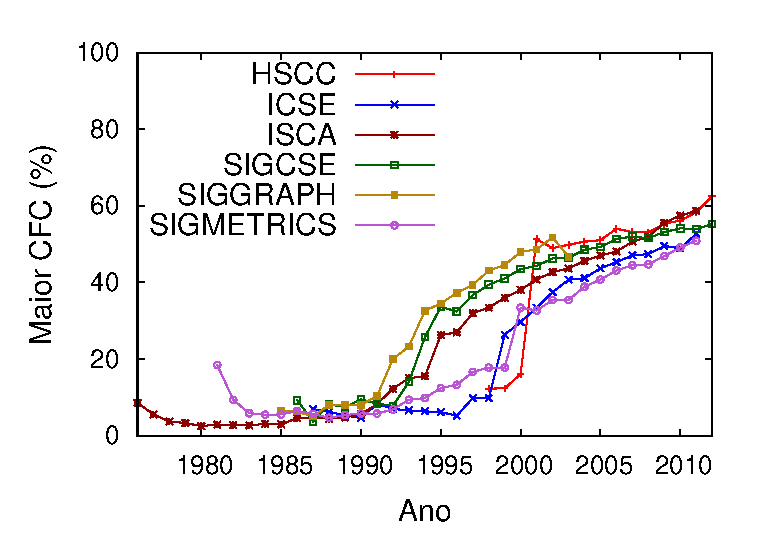
\includegraphics[scale=.6]{../graficos/sigs_metricas_acumuladas_1_em_1_ano/pt_BR/porcentagem_maior_componente_grupo_temporal_web_apendice_3.eps}
  }%
  \subfloat[Maior CFC por janela - Grupo C]{%
    \label{fig:average_shortest_slide_window_apendice_grupa_c}
    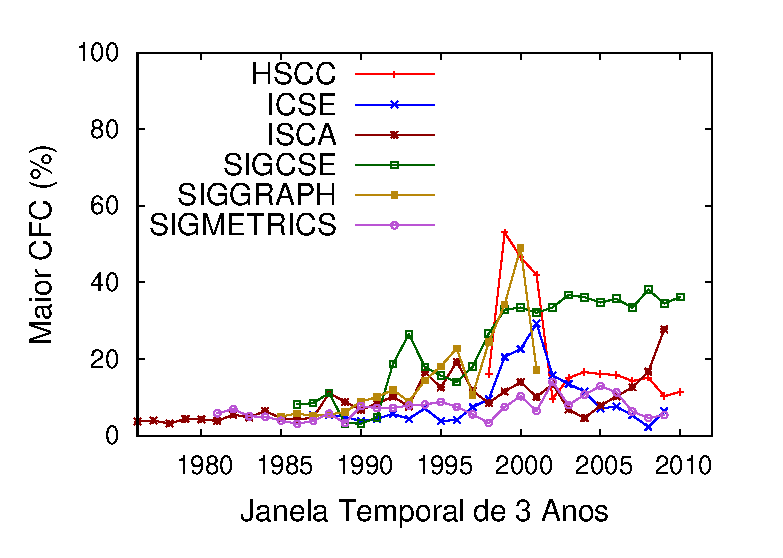
\includegraphics[scale=.6]{../graficos/core_over_time/metricas_tradicionais/pt_BR/porcentagem_maior_componente_slide_window_grupo_temporal_web_apendice_3.eps}
  }%
  \end{center}
  \caption{Maior CFC das comunidades científicas}
  \label{fig:metrics_average_shortest_apendice}
\end{figure}


\begin{figure}[!htb]
  \begin{center}
  \subfloat[Grau médio final - Grupo A]{%
    \label{fig:average_shortest_1_in_1_apendice_grupa_a}
    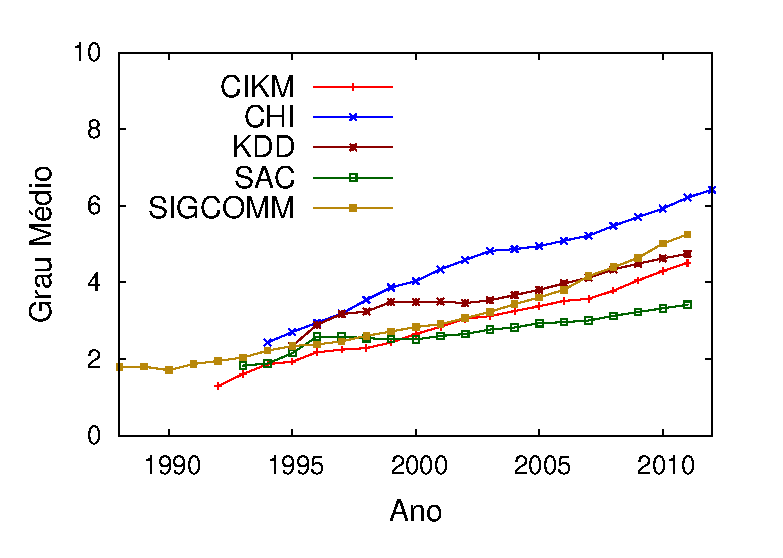
\includegraphics[scale=.6]{../graficos/sigs_metricas_acumuladas_1_em_1_ano/pt_BR/grau_medio_nodos_grupo_temporal_web_apendice_1.eps}
  }%
  \subfloat[Grau médio por janela - Grupo A]{%
    \label{fig:average_shortest_slide_window_apendice_grupa_a}
    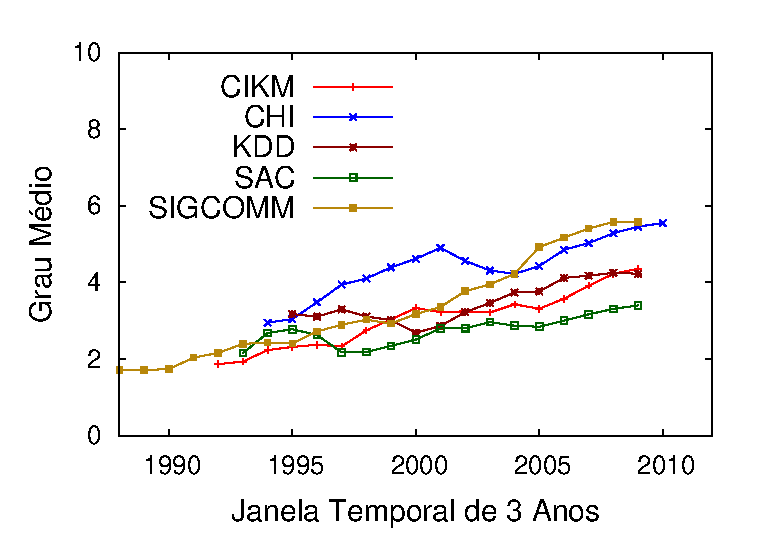
\includegraphics[scale=.6]{../graficos/core_over_time/metricas_tradicionais/pt_BR/grau_medio_nodos_slide_window_grupo_temporal_web_apendice_1.eps}
  }%
  \phantomcaption
  \end{center}
\end{figure}
\begin{figure}[!htb]
  \begin{center}
  \ContinuedFloat
  \subfloat[Grau médio final - Grupo B]{%
    \label{fig:average_shortest_1_in_1_apendice_grupa_b}
    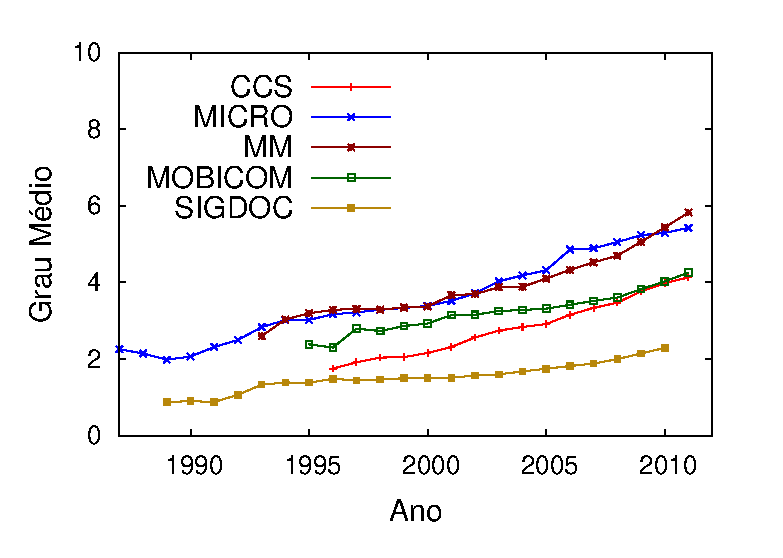
\includegraphics[scale=.6]{../graficos/sigs_metricas_acumuladas_1_em_1_ano/pt_BR/grau_medio_nodos_grupo_temporal_web_apendice_2.eps}
  }%
  \subfloat[Grau médio por janela - Grupo B]{%
    \label{fig:average_shortest_slide_window_apendice_grupa_b}
    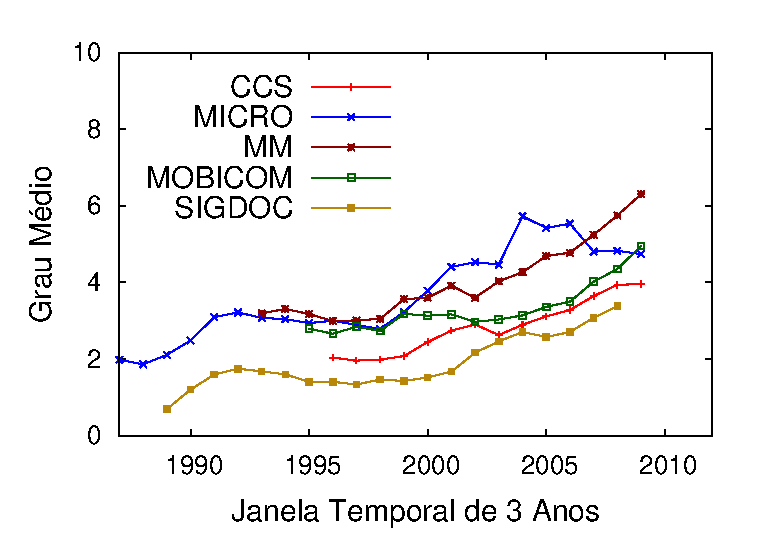
\includegraphics[scale=.6]{../graficos/core_over_time/metricas_tradicionais/pt_BR/grau_medio_nodos_slide_window_grupo_temporal_web_apendice_2.eps}
  }%
  \\
  \subfloat[Grau médio final - Grupo C]{%
    \label{fig:average_shortest_1_in_1_apendice_grupa_c}
    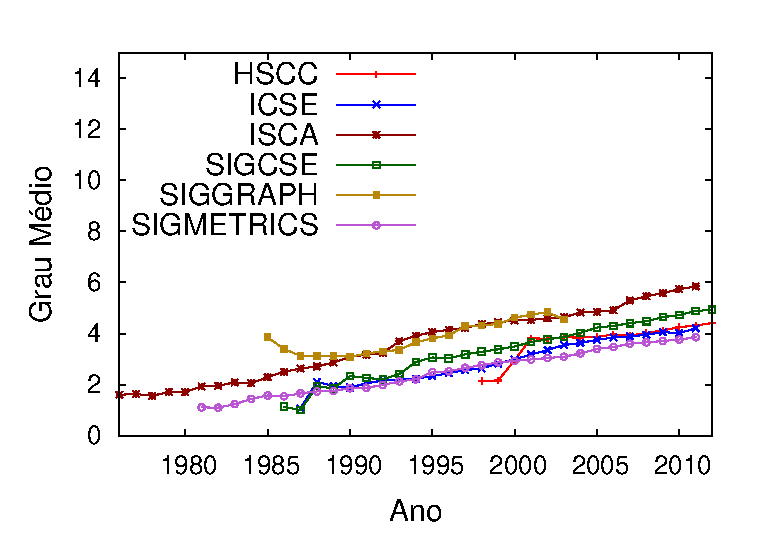
\includegraphics[scale=.6]{../graficos/sigs_metricas_acumuladas_1_em_1_ano/pt_BR/grau_medio_nodos_grupo_temporal_web_apendice_3.eps}
  }%
  \subfloat[Grau médio por janela - Grupo C]{%
    \label{fig:average_shortest_slide_window_apendice_grupa_c}
    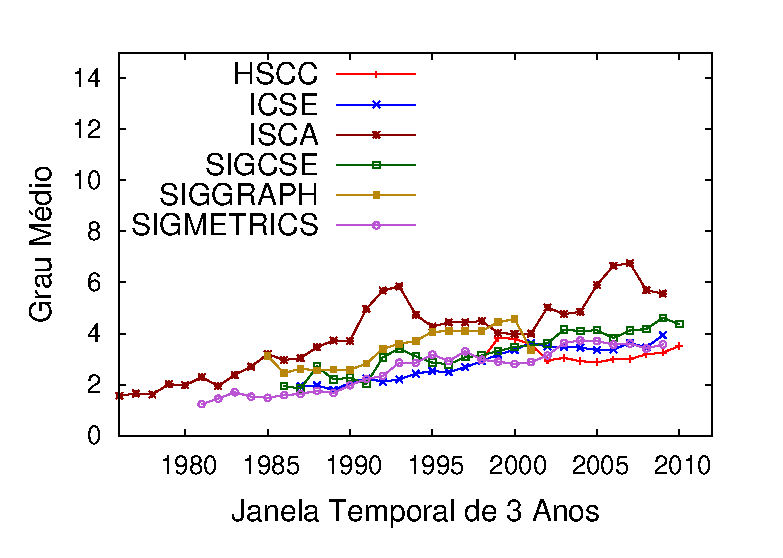
\includegraphics[scale=.6]{../graficos/core_over_time/metricas_tradicionais/pt_BR/grau_medio_nodos_slide_window_grupo_temporal_web_apendice_3.eps}
  }%
  \end{center}
  \caption{Grau médio das comunidades científicas}
  \label{fig:metrics_average_shortest_apendice}
\end{figure}